\chapter{Implementation of the model}\label{ch:3-implementation}
\markboth{Implementation of the model}{}

All the code developed for this project is available on the \href{https://github.com/MPoLS-lab/villegas-morral-msc-thesis}{Multiscale Physics of Living Systems Group's GitHub \footnote{https://github.com/MPoLS-lab/villegas-morral-msc-thesis}} and on my \href{https://github.com/villegas-morral/masters-thesis}{personal GitHub} \footnote{https://github.com/villegas-morral/masters-thesis}, and the system specifications are detailed in Section \ref{sec:specs}.

This chapter outlines the framework used to program the processes described in Chapter \ref{ch:2-abm}, details some algorithms and gives computational insight of the system. The model consists of two parts: it simulates the motion of the cells solving Equation \ref{eq:motion} using numerical methods and reproduces the state transitions as a stochastic process.



\section[Computational framework and numerical methods]{Computational framework and numerical \\ methods}


\subsection{Framework}

The code has been created using the Julia package for multicellular agent-based modelling \href{https://github.com/dsb-lab/CellBasedModels.jl}{CellBasedModels.jl} \footnote{https://github.com/dsb-lab/CellBasedModels.jl}, developed by \cite{Torregrosa_2025}, along with the examples provided in the documentation.

A brief description of each program along with the required packages to run them can be found in Section \ref{sec:code}, and a general outline of the code is provided in Program \ref{pg:example-code}.

Note that the computational model works with dimensionless units. Once the simulations are finished, these can be converted to extract and plot the data in physical units.


\subsection{Integration of the equations of motion}

The method chosen to solve the equations of motion for each cell is Heun's method, which can be derived from Euler's method \parencite{Suli_2003,Brorson_2022}. Consider the following differential equation,
$$\frac{\diff x}{\diff t} = v(t,x).$$

Given a timestep $\Delta t$ and a number of steps $l$, its solution is approximated by the discrete function $\{x_n\}_{n=0,\dots,l}$ defined over $\{t_n\}_{n=0,\dots,l}$ such that
$$x_n\approx x(t_n), \quad\quad t_{n1}-t_n=\Delta t.$$
The values $x_0$, $v_0$ at time $t_0$ follow from the initial condition.

In the forward Euler method, the rest of the values are approximated by taking
\begin{equation}
    x_{n+1}=x_n+ v(t_n,x_n)\Delta t,
\end{equation}
while in the backward Euler method, they follow from
\begin{equation}\label{eq:backward}
    x_n=x_{n+1}-v(t_{n+1},x_{n+1})\Delta t.
\end{equation}

Heun's method is a simple predictor-corrector method which combines these two:

\begin{enumerate}
    \item Compute $x_n$ and $v(t_n,x_n)$.
    \item Compute an initial prediction $x_{n+1,p}$ using the forward Euler method,
        $$x_{n+1,p}=x_n+ v(t_n,x_n)\Delta t.$$
    \item Isolate $x_{n+1}$ in Equation \ref{eq:backward} and compute the corrector $x_{n+1,c}$ according to the backward Euler method using the predictor $x_{n+1,p}$ obtained in the previous step,
        $$x_{n+1,c}= x_n +v(t_{n+1},x_{n+1,p})\Delta t.$$
    \item The final approximation $x_{n+1}$ is the average,
        \begin{align}
            \begin{aligned}
                x_{n+1} = x_n + \frac{\Delta t}{2} \left(v(t_n,x_n)+v(t_{n+1},x_{n+1,p})\right).
            \end{aligned}
        \end{align}
\end{enumerate}


\subsection{Algorithm for cell differentiation}

Given probabilities $p,q$ as described in Definition \ref{def:constant-rates}, cell differentiation for an arbitrary cell $i$ follows the next rules for each timestep $\Delta t$.
\begin{enumerate}
    \item If the evolution of states is turned off or $\text{state}(i)=C$, stop.
    \item Count the proportion of neighbours in state $A$, that is, $\langle\mathds{1}_A(i)\rangle$.
    \item If $\text{state}(i)=A$
    \begin{enumerate}[label=\roman*.]
        \item Compute $r_{A\rightarrow B}$.
        \item Choose $\xi \rightarrow \text{U}(0,1)$.
        \item If $\xi < r_{A\rightarrow B}\Delta t$, then cell $i$ transitions and $\text{state}(i)=B$.
    \end{enumerate}
    \item If $\text{state}(i)=B$
    \begin{enumerate}[label=\roman*.]
        \item Compute $r_{B\rightarrow C}$.
        \item Choose $\xi \rightarrow \text{U}(0,1)$.
        \item If $r<r_{B\rightarrow C}\Delta t$, then cell $i$ transitions and $\text{state}(i)=C$.
    \end{enumerate}
\end{enumerate}



\section[Numerical validation of the global friction approximation]{Numerical validation of the global friction \\ approximation}

This section outlines the procedures followed to obtain a functional and efficient computational model, focusing on the validation of the friction approximation stated in Equation \ref{eq:globalfriction}.


\subsection{Aggregate stability}

Some parameters can induce numerical errors if not tuned appropriately. For example, when a cell in the outer layer divides, the cells that were in contact with the mother cell may detach from the aggregate due to numerical errors (see Figure \ref{fig:aggregate_broken}). In order to obtain a stable aggregate, we will adjust the timestep ($\Delta t$), the overlap parameter ($\alpha_\text{ov}$), and the friction coefficient ($\lambda$). 

The stability of a parameter can be tested using Program \ref{pg:formed-correctly}, which implements a function that returns whether the aggregate consists of a single connected component.

\begin{figure}[ht]
    \centering
    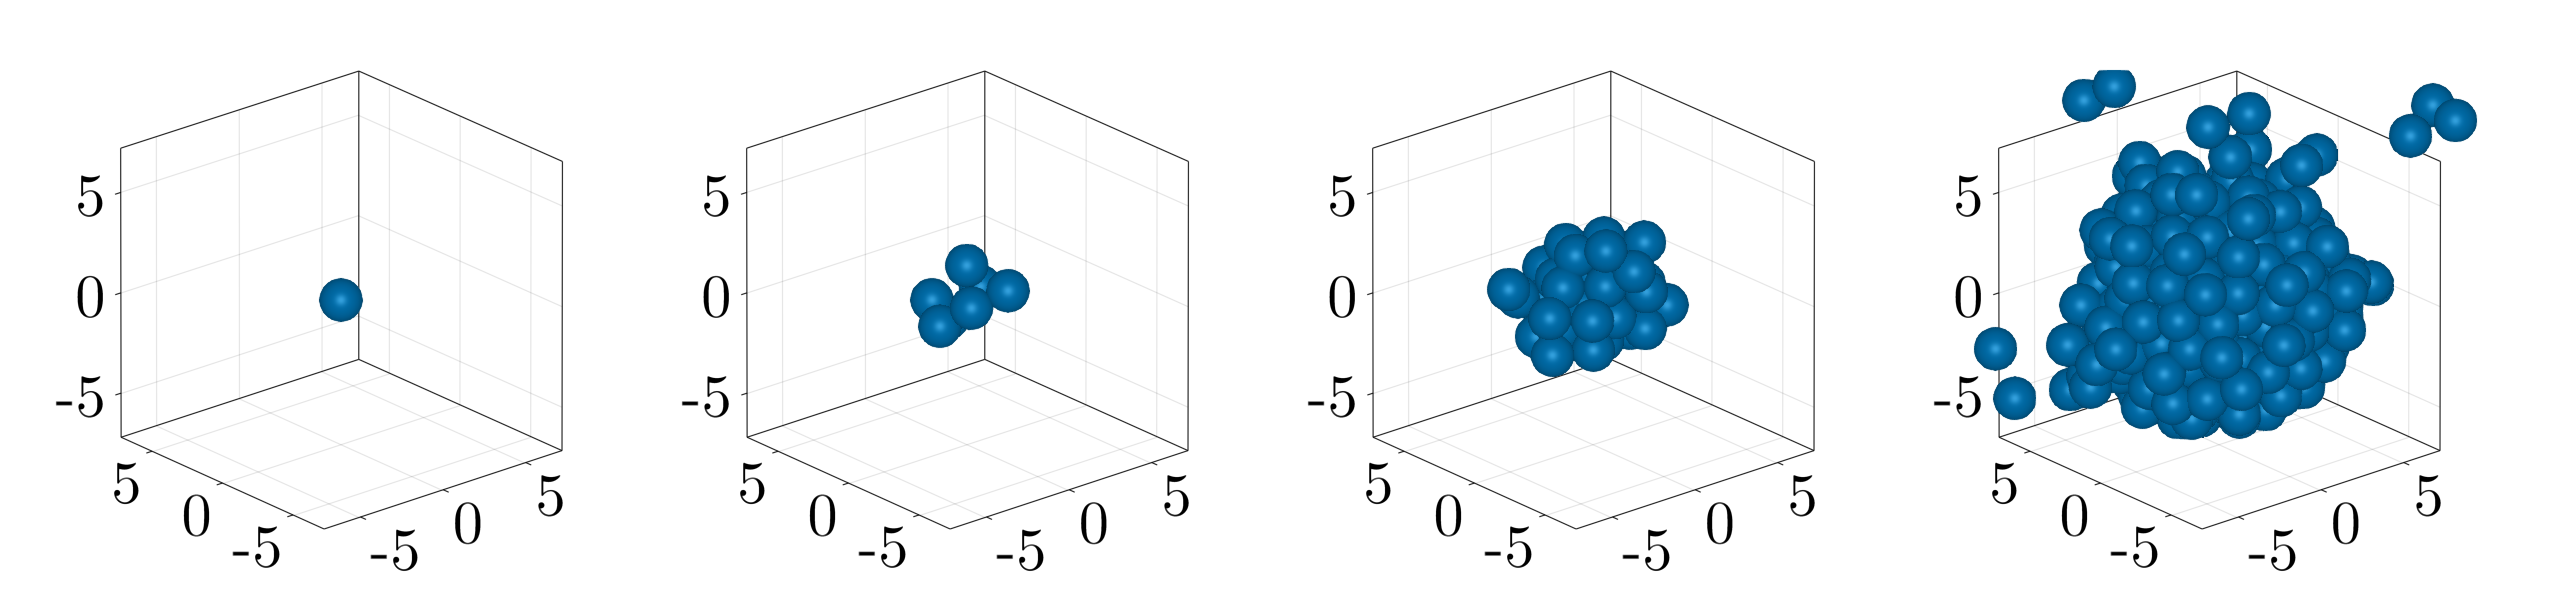
\includegraphics[width=\textwidth]{figures/400/400-aggregate-broken.png}
    \caption{Unstable simulation.}
    \label{fig:aggregate_broken}
\end{figure}

Complex models often require smaller timesteps, which increase computational costs. Balancing this trade-off between model complexity and computational efficiency is essential for creating an effective model.

During cell division, two daughter cells emerge from a mother cell. The overlap factor determines how closely these daughter cells are placed in the aggregate after the mother cell is removed. This simplification accounts for the repulsion force between these cells before they completely split, so that we can modify $\alpha_\text{ov}$ freely.

Since we are simulating \textit{in vitro} cell cultures, the physical parameters could be in principle measured. In our study, friction accounts for the binding and unbinding connecting neighbouring cells.

Next, we focus on the stability of the aggregate formation, turning off differentiation. Since cell rearrangements are not relevant, we simplify the computations by setting active protrusions to zero ($F_{p_i}=0$).


\subsection{Global friction and average number of neighbours}\label{sec:avg_nbs}

The aim of this section is to analyse the average number of neighbours in the system in order to identify and correct potential issues, and to compute an approximation for it. This leads to the expression selected for $F_{ij}$ in Equation \ref{eq:fij}.

Let $N(t)$ denote the total number of agents in the system, and $\langle n_i \rangle (t)$ denote the average the number of neighbours of a cell over time,
\begin{equation}
    \langle n_i \rangle (t) = \frac{1}{N(t)}\sum_{i=1}^N{n_i(t)}.
\end{equation}

We consider a simpler (see Equation \ref{eq:fij}) force profile for $F_{ij}$ that will be polished after the analysis,
\begin{equation}\label{eq:badforce}
    F_{ij}= 
    \begin{dcases}
        \frac{(x_i-x_j)}{d_{ij}}F_0 f_r(d_{ij})\alpha_\text{adh}
        &\quad \text{if $d_{ij} < 2\mu r$}        \\
        0 &\quad \text{otherwise.}
    \end{dcases}
\end{equation}

The final equations of motion presented in Chapter \ref{ch:2-abm} assume the simplification
\begin{equation}\tag{\ref{eq:globalfriction}}
    \Lambda n_i(t)\equiv \lambda>0,
\end{equation}
presented in Section \ref{sec:simplify}. The value for $\lambda$ will be chosen using $\langle n_i \rangle$.

Therefore, in this section we consider the following equations of motion,
\begin{align}\label{eq:motion_variable}
    \begin{aligned}
        \Lambda n_i v_i &= \sum_{j=1}^{N} F_{ij}\\
        \frac{\diff x_i}{\diff t} &=v_i.
    \end{aligned}
\end{align}
Note that we are not addressing the absence of net flows yet, presented in Equation \ref{eq:netflows} before the global friction. For convenience, this is discussed in the next section (\ref{sec:vsum-zero}).

Since the computational implementation uses the dimensionless form of the equations, the typical value of the friction coefficient $\tilde\Lambda n_i$ is expected to be of the order of $1$. The number of neighbours should be of the order of $10$, so we set $\tilde\Lambda=0.1$. 


\subsubsection*{Analysis of $\langle n_i \rangle$ over time}

During proliferation, the average number of neighbours is expected to stabilize over time. In particular, since cells in the centre of the aggregate have the maximum number of neighbours, once the distance to the outer layer is larger than the neighbour range, this number should not change.

In \code{CellBasedModels.jl}, aggregates are stored in objects which allow access to past timestamps. Using Program \ref{pg:niproblem-avg}, we grow five aggregates up to 1000 agents (see Figure \ref{fig:aggregate_clustered}), and compute $\langle n_i \rangle$ against $N(t)$. This plot is displayed in Figure \ref{fig:avg_ncells_vs_ni}.

This data shows that, in this simulation, the average number of neighbours increases with $N$ and could be roughly approximated to 
\begin{equation}\label{eq:ni_approx}
    \langle n_i \rangle (t)\approx0.1N(t).
\end{equation}

\begin{figure}[ht]
    \centering
    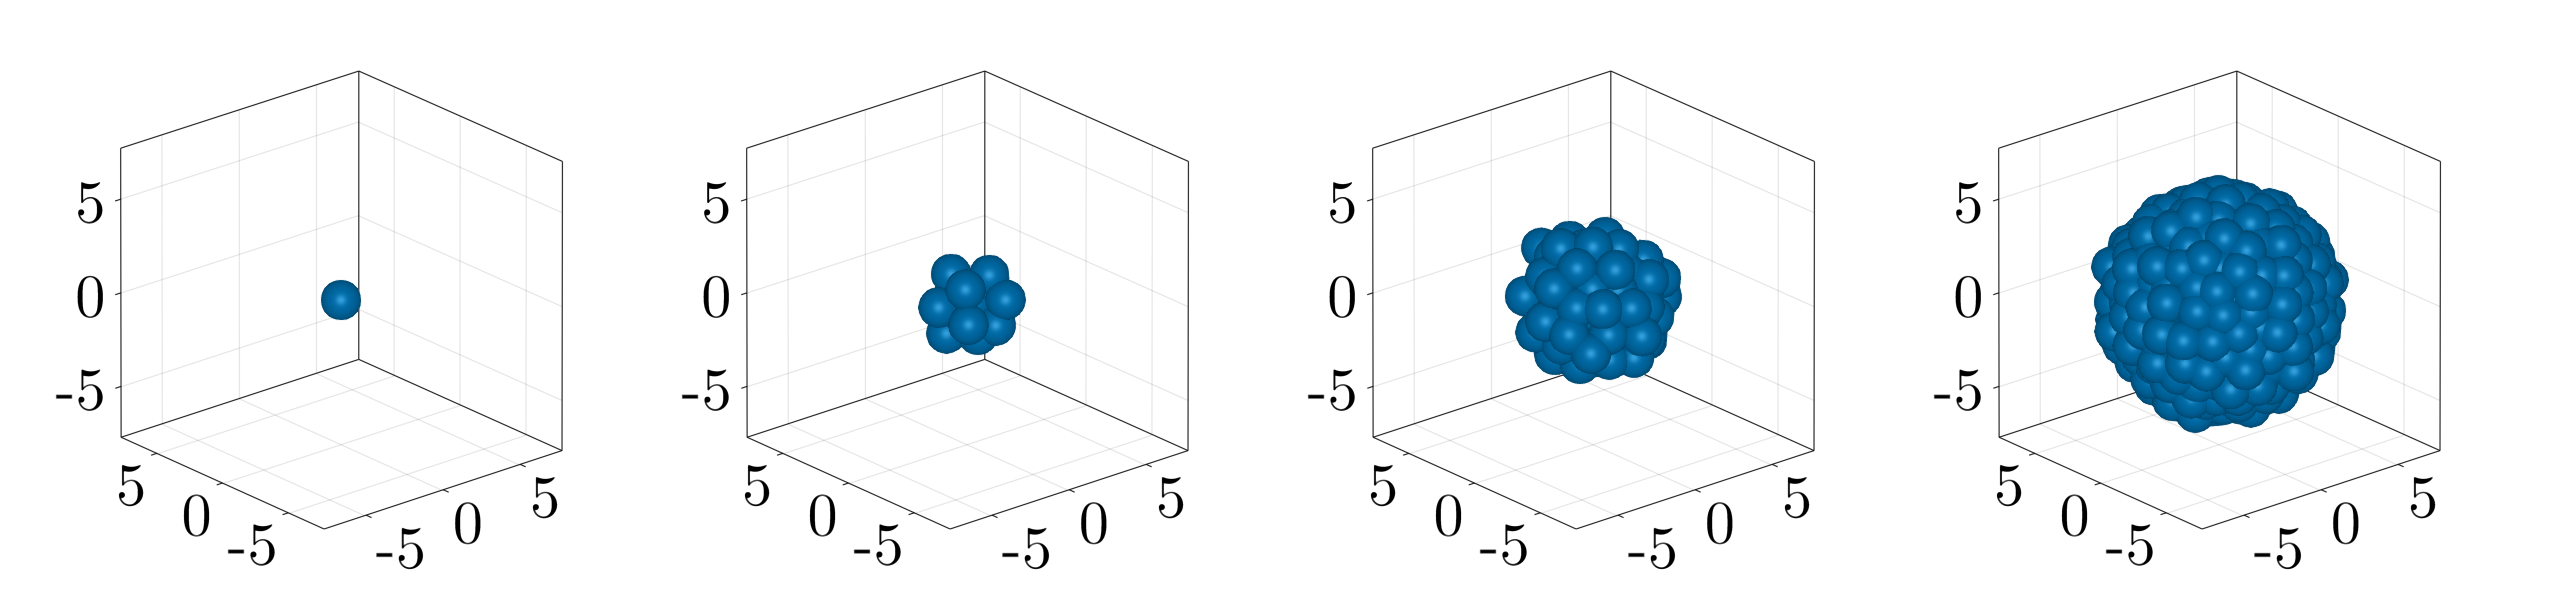
\includegraphics[width=\textwidth]{figures/301/301-aggregate-clustered.png}
    \caption{Proliferation of an aggregate using Equations \ref{eq:badforce} and \ref{eq:motion_variable}.}
    \label{fig:aggregate_clustered}
\end{figure}

\begin{figure}[ht]
    \centering
    \begin{minipage}{0.45\textwidth}
        \centering
        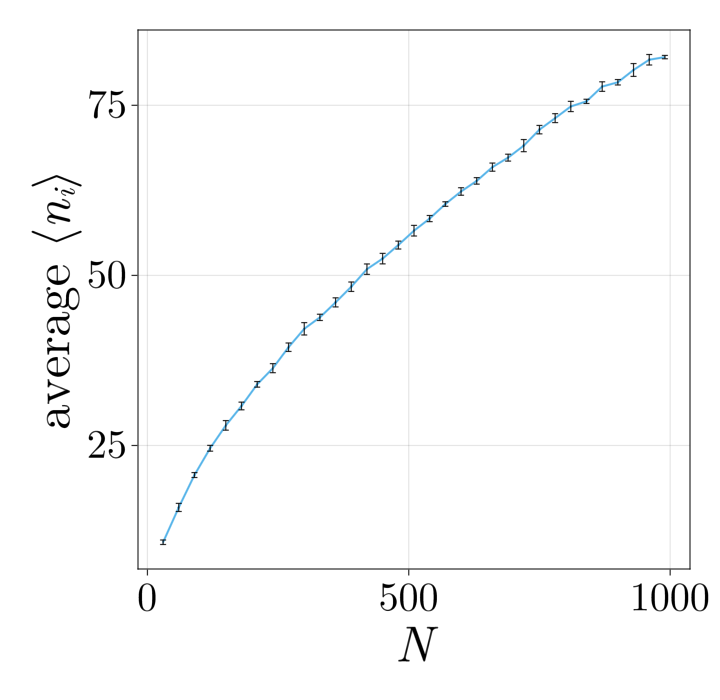
\includegraphics[width=\textwidth]{figures/301/301-ncells-vs-ni-1000.png}
    \end{minipage}
    \hspace{0.5cm}
    \begin{minipage}{0.45\textwidth}
        \centering
        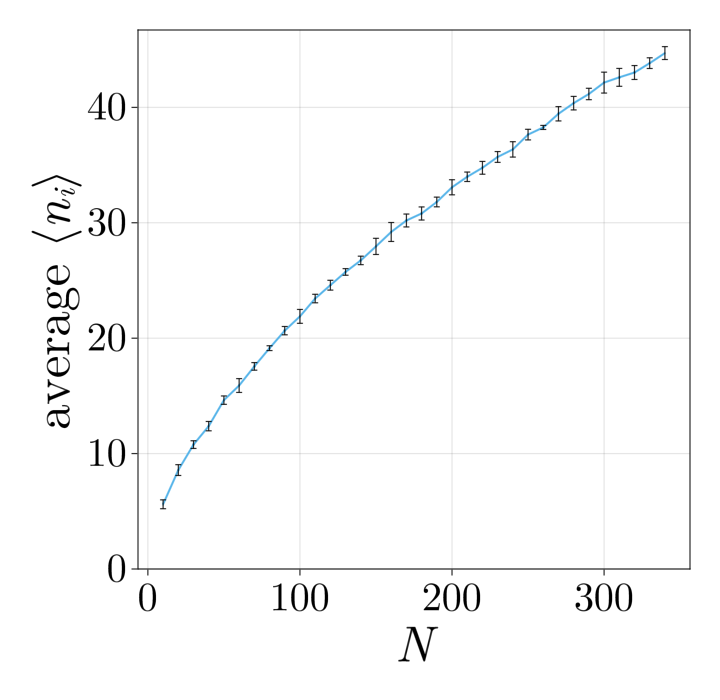
\includegraphics[width=\textwidth]{figures/301/301-ncells-vs-ni-300.png}
    \end{minipage}
    \caption{$\langle n_i\rangle$ against $N(t)$. Averaged over five realizations. Bars indicate the standard deviation of averaging the five systems.}
    \label{fig:avg_ncells_vs_ni}
\end{figure}



However, this is not what one would expect from a closely packed structure. We continue the analysis and, later in the section, propose a solution.

Henceforth, we will use Program \ref{pg:niproblem} to focus on a single realization due to the small standard deviation observed. First, we plot the number of neighbours (see Figure \ref{fig:ncells_vs_ni}).

\begin{figure}[ht]
    \centering
    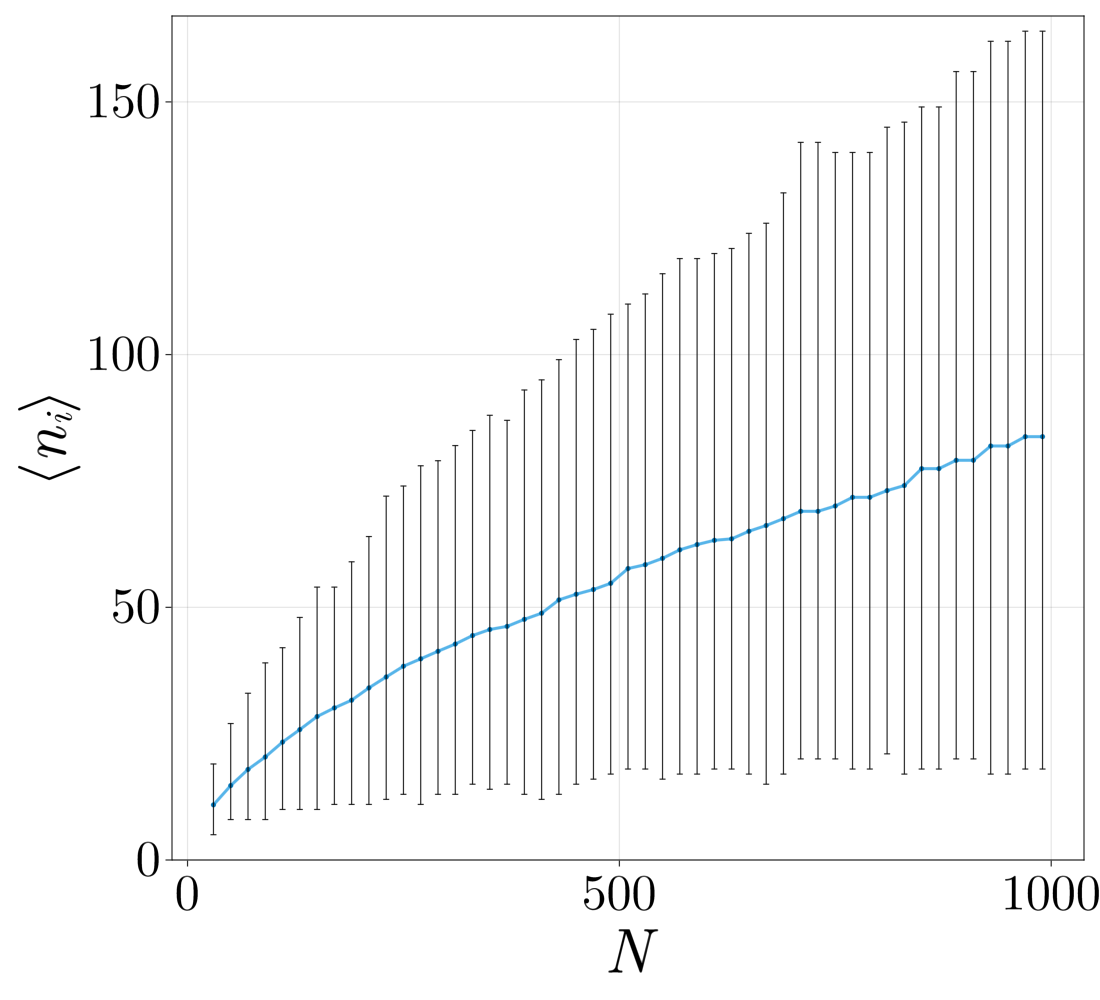
\includegraphics[width=0.5\textwidth]{figures/302/302-ncells-vs-ni_single.png}
    \caption{Average number of neighbours against $N(t)$. Bars indicate the highest and lowest number of neighbours.}
    \label{fig:ncells_vs_ni}
\end{figure}

The lowest number of neighbours, corresponding to the outer layer cells, remains constant as expected. However, it is the cells with largest $n_i$ that experience an increase in neighbours, that is, the inner cells. To visualize the issue, we plot the neighbours of the cell with the highest $n_i$ in the final timestamp alongside the aggregate itself in Figure \ref{fig:aggregate_nbs}.

\begin{figure}[ht]
    \centering
    \begin{subfigure}{0.45\textwidth}
        \centering
        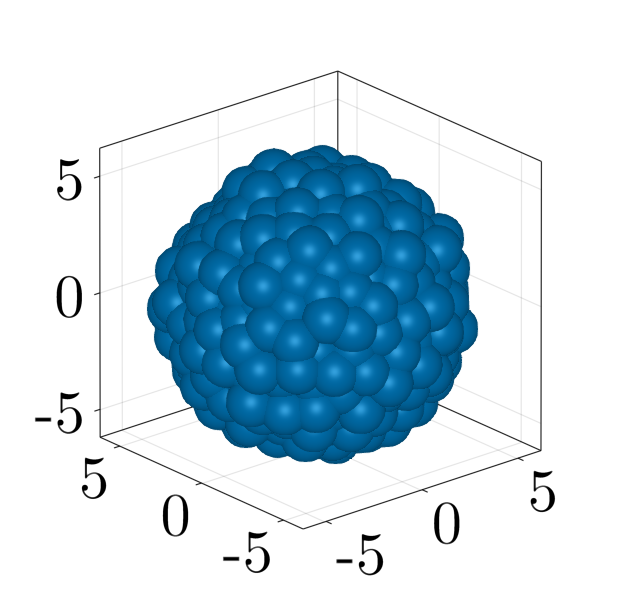
\includegraphics[width=0.65\linewidth]{figures/302/302-aggregate-nbs-full.png}
        \caption{Final aggregate. \\ \hfill}
    \end{subfigure}
    % \hfill
    \begin{subfigure}{0.45\textwidth}
        \centering
        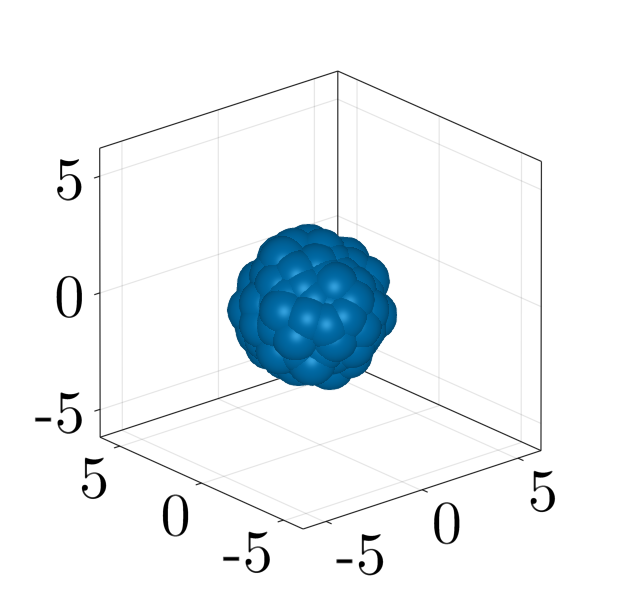
\includegraphics[width=0.65\linewidth]{figures/302/302-aggregate-nbs.png}
        \caption{Neighbours of the cell \\ with the highest $n_i$.}
    \end{subfigure}
    
    \caption{Aggregate of $N=900$ and set of $n_i=151$ neighbours.}
    \label{fig:aggregate_nbs}
\end{figure}

\newpage
The issue is that cells in the inner part of the aggregate become trapped in a dense configuration with excessive overlap, which is physically implausible. This is a common drawback when using centre-based models \parencite{Liedekerke_2015}. 


\subsubsection*{Proposed solution}

A possible way of addressing this issue can be using a different method to count neighbours, such as considering Gabriel neighbours \parencite{Oriola_2022}. If we used this method, we should either approximate $\lambda$ by Equation \ref{eq:ni_approx} depending on the magnitude of the aggregates to simulate, or use the model with variable friction $n_i \Lambda$.

Decreasing the proliferation rate to allow cells to relax and accommodate with less overlap does not resolve the problem either. To ensure that cells are able to reorganize during the differentiation process, we instead propose a change in the force profile to prevent excessive overlap.

In the definition for $F_{ij}$ stated in Equation \ref{eq:badforce}, the expression for the attractive and the repulsive regimes described in Remark \ref{rk:regimes} is the same. Still, repulsion forces are not enough to separate the cells overlapped in the centre. We thus consider a force profile that splits the two regimes and controls the difference in strength through a repulsion factor,
\begin{equation}\tag{\ref{eq:fij}}
    F_{ij}= 
    \begin{dcases}
        \frac{(x_i-x_j)}{d_{ij}} 
        F_0 f_r(d_{ij})\alpha_\text{adh}\alpha_\text{rep}
        &\quad \text{if $d_{ij}\leq 2 r$} \\
        \frac{(x_i-x_j)}{d_{ij}}
        F_0 f_r(d_{ij}) \alpha_\text{adh}
        &\quad \text{if $2r<d_{ij}<2\mu r$} \\
        0 &\quad \text{otherwise,}
    \end{dcases}
\end{equation}

Next, we look for an appropriate repulsion factor using Program \ref{pg:solution-varfriction}. Recall that, for $\alpha_\text{rep}=1$, we recover the force expression from Equation \ref{eq:badforce}.

Our final aim is to reliably simulate aggregates of the magnitude of 500 cells, so we consider a system of $N=800$. Varying $\alpha_\text{rep}\in\{1,2,2.5,3\}$, the cells with the highest $n_i$ have, respectively, 142, 45, 30 and 25 neighbours. These neighbourhoods and the aggregates they belong to are shown in Figure \ref{fig:aggregates_reps}.

\begin{figure}[ht]
    \centering
    \begin{subfigure}{\textwidth}
        \centering
        \begin{subfigure}{0.22\textwidth}
            \centering
            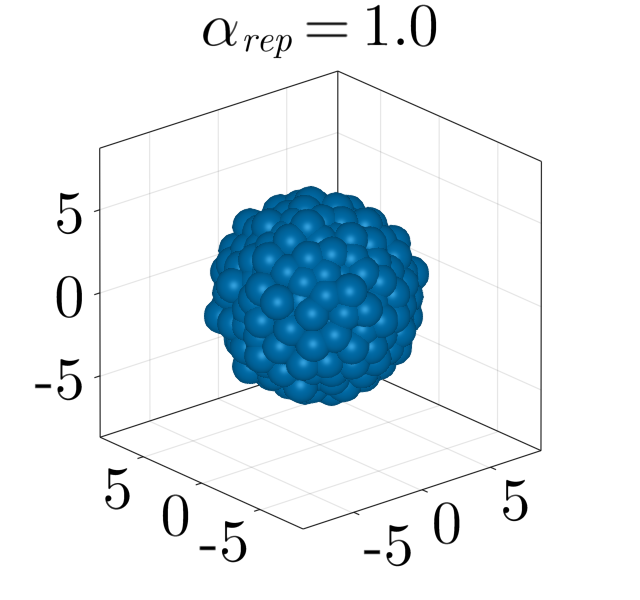
\includegraphics[width=\textwidth]{figures/303/303-aggregates-reps-1.png}
        \end{subfigure}
        \hfill
        \begin{subfigure}{0.22\textwidth}
            \centering
            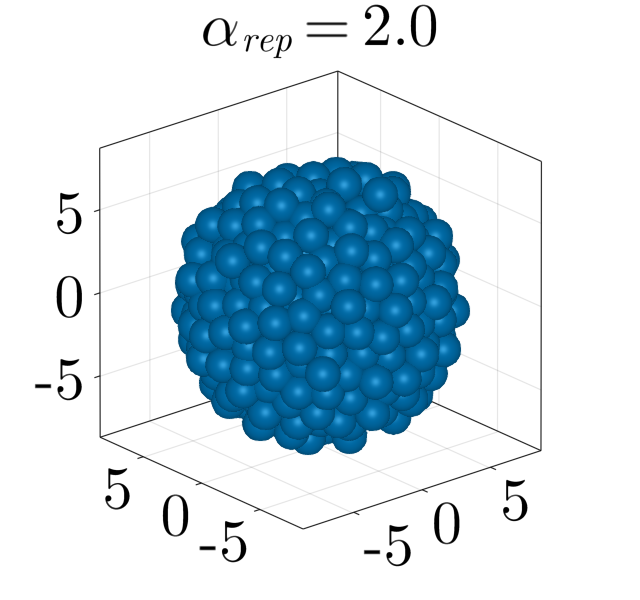
\includegraphics[width=\textwidth]{figures/303/303-aggregates-reps-2.png}
        \end{subfigure}
        \hfill
        \begin{subfigure}{0.22\textwidth}
            \centering
            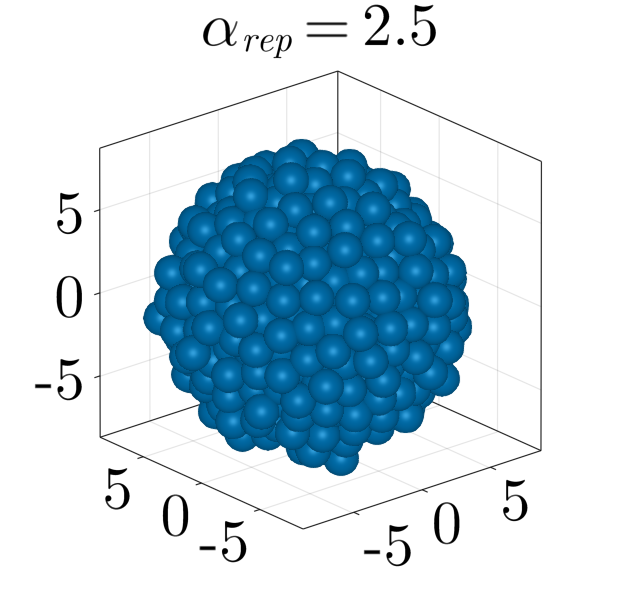
\includegraphics[width=\textwidth]{figures/303/303-aggregates-reps-2dot5.png}
        \end{subfigure}
        \hfill
        \begin{subfigure}{0.22\textwidth}
            \centering
            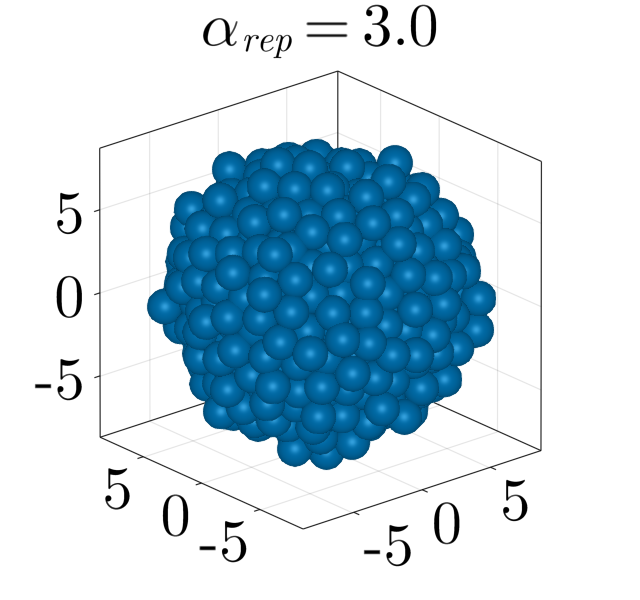
\includegraphics[width=\textwidth]{figures/303/303-aggregates-reps-3.png}
        \end{subfigure}
        \caption{Final aggregate.}
    \end{subfigure}
    \vspace{0.5em}
    \begin{subfigure}{\textwidth}
        \centering
        \begin{subfigure}{0.22\textwidth}
            \centering
            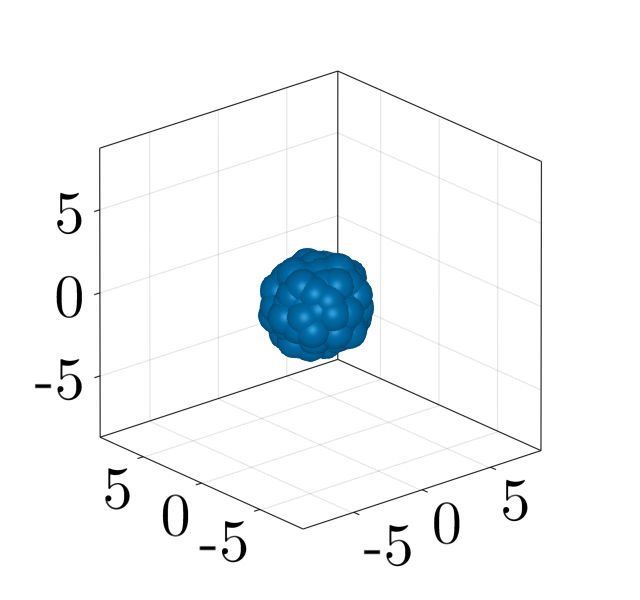
\includegraphics[width=\textwidth]{figures/303/303-aggregates-reps-nbs-1.png}
        \end{subfigure}
        \hfill
        \begin{subfigure}{0.22\textwidth}
            \centering
            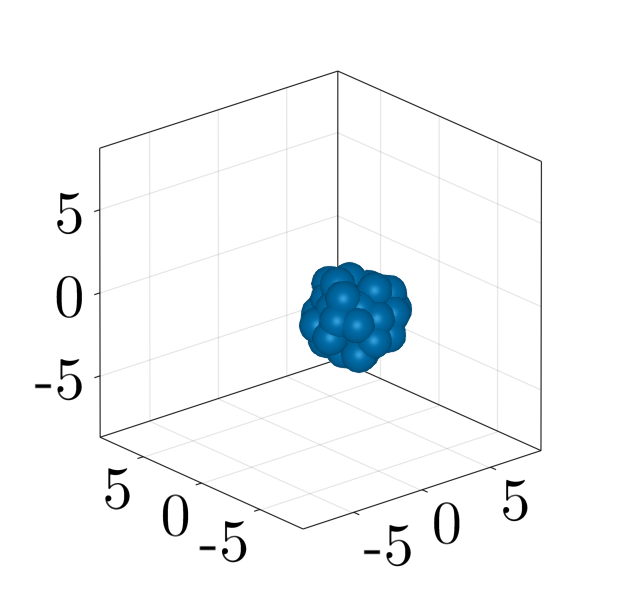
\includegraphics[width=\textwidth]{figures/303/303-aggregates-reps-nbs-2.png}
        \end{subfigure}
        \hfill
        \begin{subfigure}{0.22\textwidth}
            \centering
            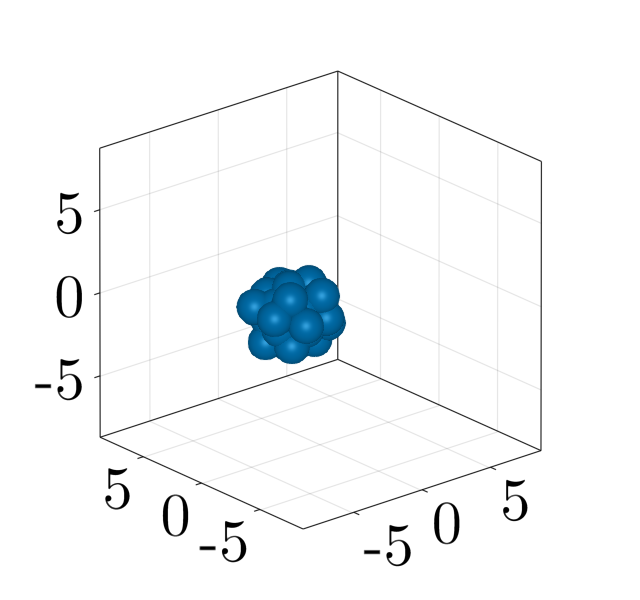
\includegraphics[width=\textwidth]{figures/303/303-aggregates-reps-nbs-2dot5.png}
        \end{subfigure}
        \hfill
        \begin{subfigure}{0.22\textwidth}
            \centering
            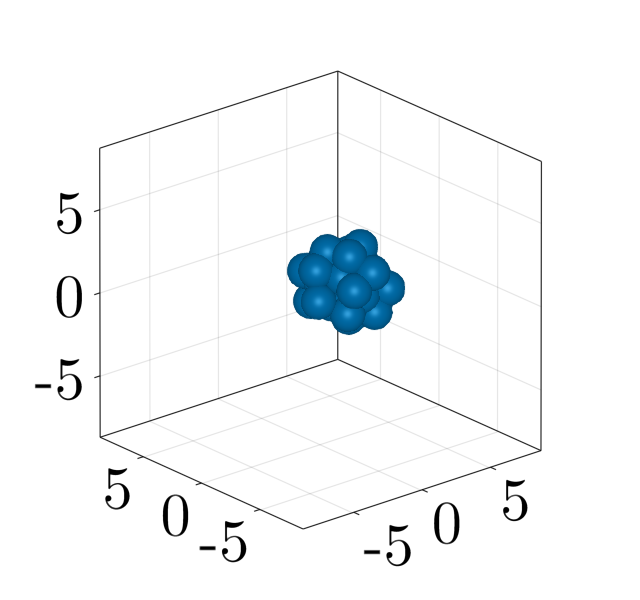
\includegraphics[width=\textwidth]{figures/303/303-aggregates-reps-nbs-3.png}
        \end{subfigure}
        \caption{Largest neighbourhood for each aggregate.}
    \end{subfigure}
    \caption{Aggregates and sets of neighbours by varying $\alpha_\text{rep}$.}
    \label{fig:aggregates_reps}
\end{figure}

Figure \ref{fig:reps_ni_vs} illustrates the average number of neighbours in terms of the number of cells. Values $\alpha_\text{rep}\in\{2.5,3\}$ yield the best results. The averages of neighbours are approximated as their average over time,
\begin{equation}
    \begin{aligned}
        \langle n_i\rangle(t)_{2.5}&\approx 8 \pm 5,\\
        \langle n_i\rangle(t)_{3.0}&\approx 7 \pm 4
    \end{aligned}
\end{equation}

We determine to set $\alpha_\text{rep}=2.5$ when simplifying the model using global friction (see Program \ref{pg:proposal}), given that it is the lowest factor that offers a realistic output, and approximate $\langle n_i \rangle(t)\approx10$, thus considering the friction coefficient
\begin{equation}
    \tilde\lambda = 10\tilde\Lambda = 0.1.
\end{equation}

To further discourage the possibility that cells cluster because of a numerical problem during development, we tried setting $\alpha_\text{rep}=1$ in an aggregate grown using $\alpha_\text{rep}=2.5$. The aggregate rapidly compressed (see Figure \ref{fig:aggregate_revert}), proving that $\alpha_\text{rep}=\alpha_\text{atr}=1$ are not feasible in this model.

\begin{figure}[ht]
    \centering
    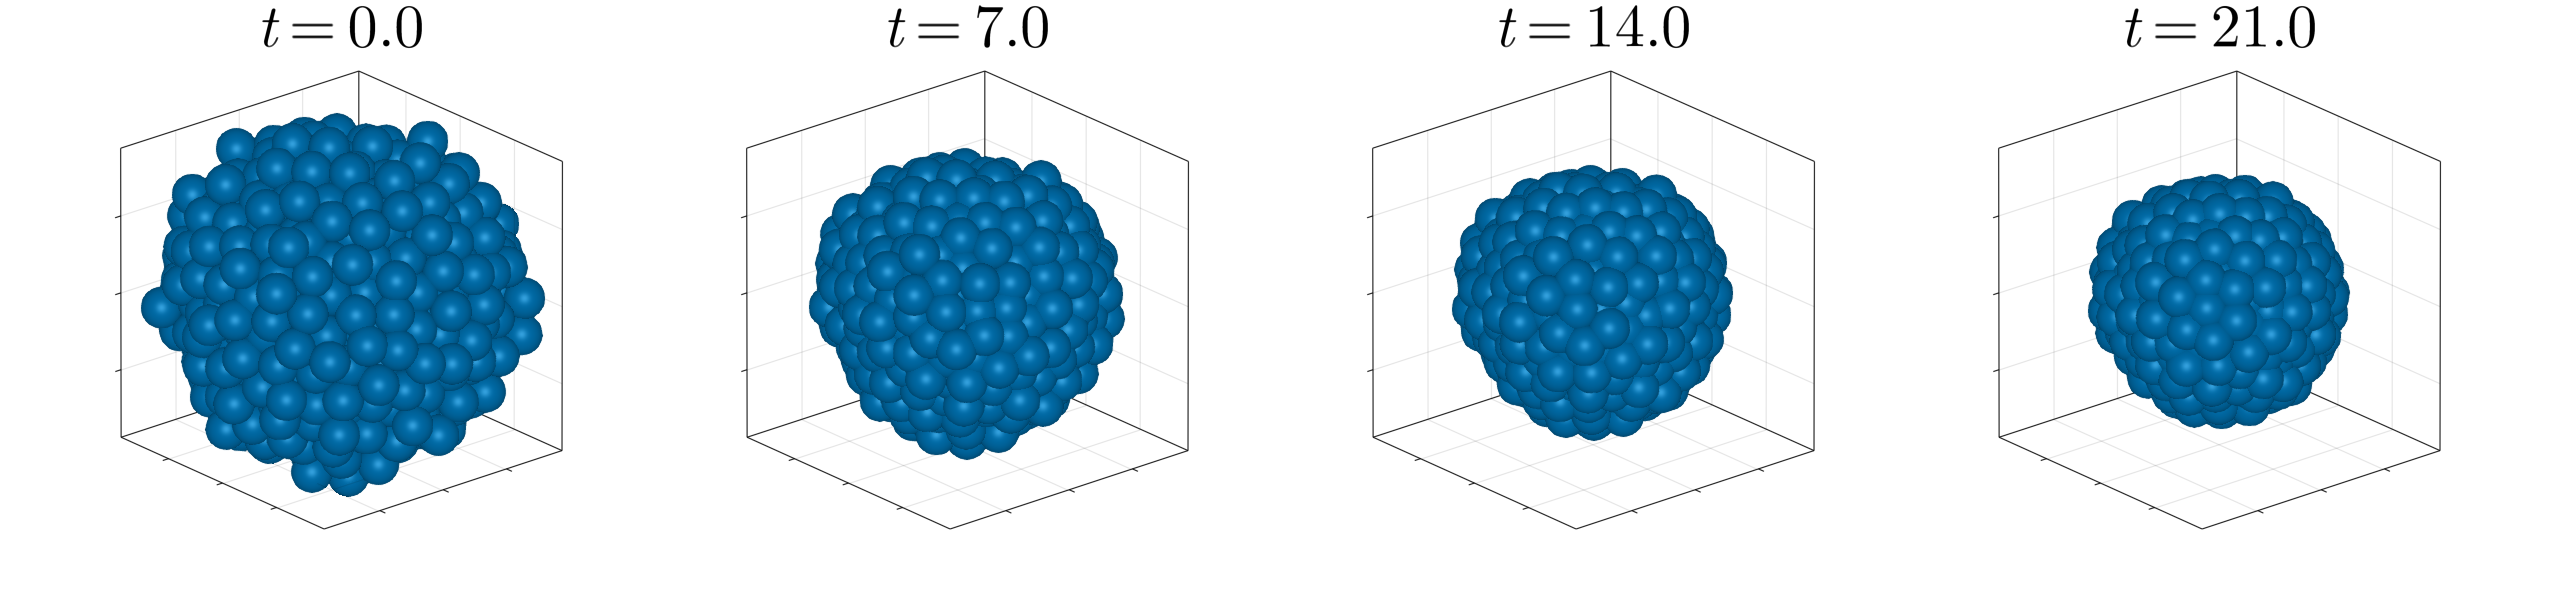
\includegraphics[width=0.8\textwidth]{figures/303/303-aggregate-revert-titles.png}
    \caption{Changing $\alpha_\text{rep}$ from 2.5 to 1.}
    \label{fig:aggregate_revert}
\end{figure}

Finally, the protrusion force is also split into repulsive and attractive regimes,
\begin{equation}\tag{\ref{eq:fij}}
    F_{p_i}=
    \begin{dcases}
        - \frac{(x_i-x_j)}{d_{ij}} D \alpha_\text{rep}
        &\quad \text{if $d_{ij}\leq 2 r$} \\
        - \frac{(x_i-x_j)}{d_{ij}} D
        &\quad \text{if $2r<d_{ij}<2\mu r$}.
    \end{dcases}
\end{equation}

The appropriate implementation of this factor is addressed in Section \ref{sec:protrusion-force}.


\subsection{Absence of net flows}\label{sec:vsum-zero}

This section tests using different approaches the assumption that net flows are negligible,
\begin{equation}\tag{\ref{eq:netflows}}
    \sum_{j\in U_i}v_j\approx 0.
\end{equation}

First, we simulate the system using the equations of motion before the approximation,
\begin{align}\label{eq:worst}
    \begin{aligned}
        \Lambda n_i v_i &=\Lambda\sum_{j\in U_i}v_j+\sum_{j=1}^{N} F_{ij} + P_i F_{p_i}\\
        \frac{\diff x_i}{\diff t} &=v_i,
    \end{aligned}
\end{align}
However, when including the sum of velocities term, our code turns out to be numerically unstable (see Program \ref{pg:unstable-vsum}).

The simplification consists of removing the weight of the sum of velocities from the equations of motion, but it does not actually set this term to be zero. Therefore, testing Hypothesis \ref{eq:netflows} with the model with variable friction proposed in Program \ref{pg:solution-varfriction} is still significant. Program \ref{pg:vsum-zero} verifies that the expression is indeed null. 

\begin{figure}[p]
    \centering
    \begin{minipage}{0.49\textwidth}
        \centering
        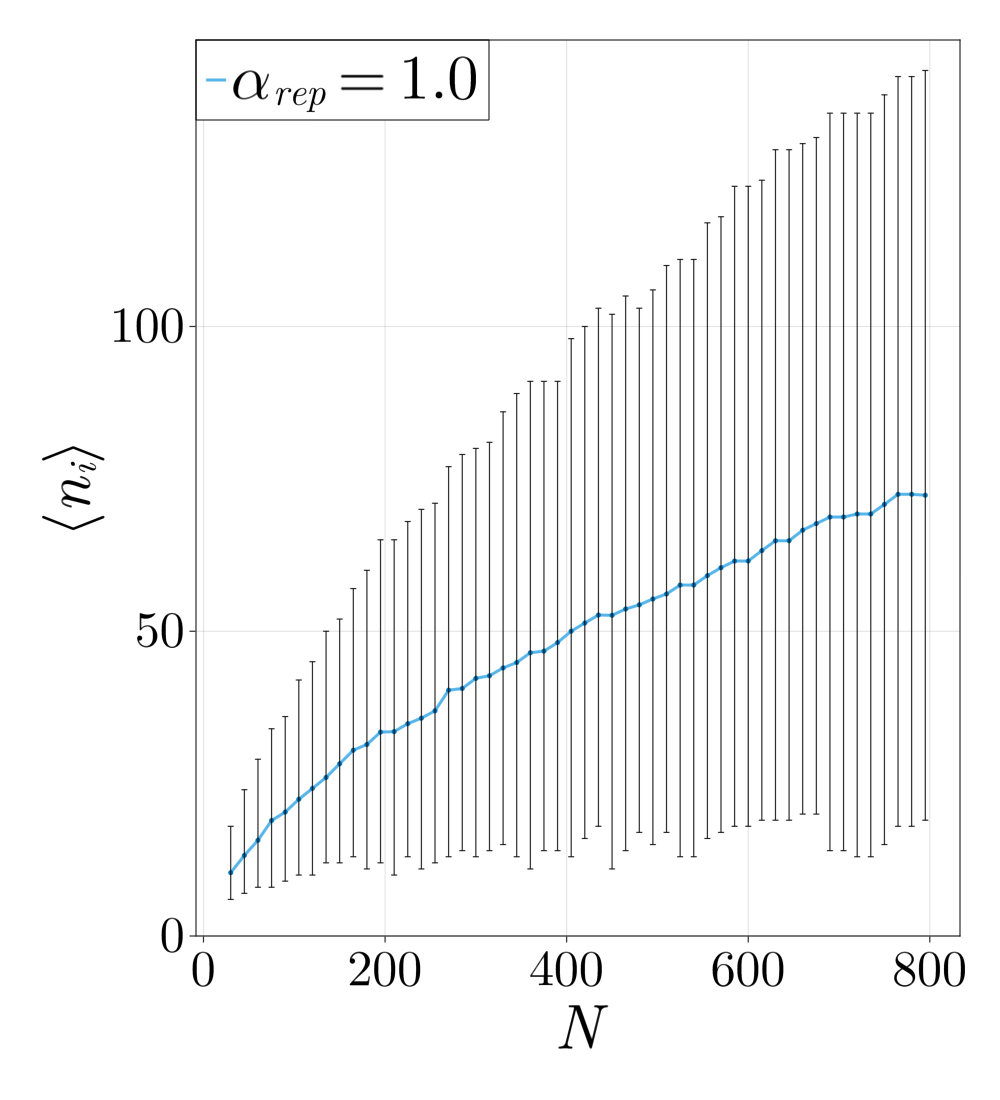
\includegraphics[width=\linewidth]{figures/303/303-reps-ni-1.png} 
    \end{minipage}
    \begin{minipage}{0.49\textwidth}
        \centering
        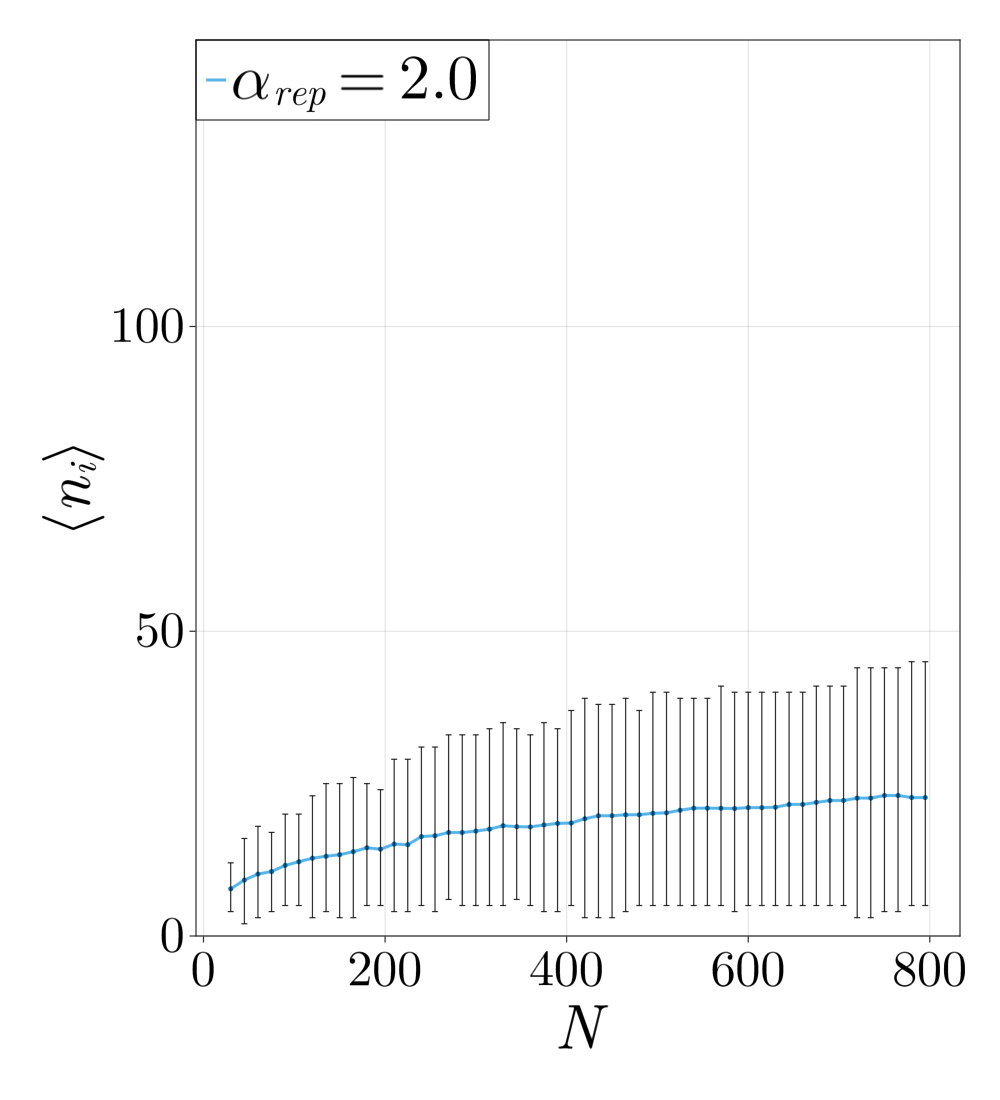
\includegraphics[width=\linewidth]{figures/303/303-reps-ni-2.png} 
    \end{minipage}
    \begin{minipage}{0.49\textwidth}
        \centering
        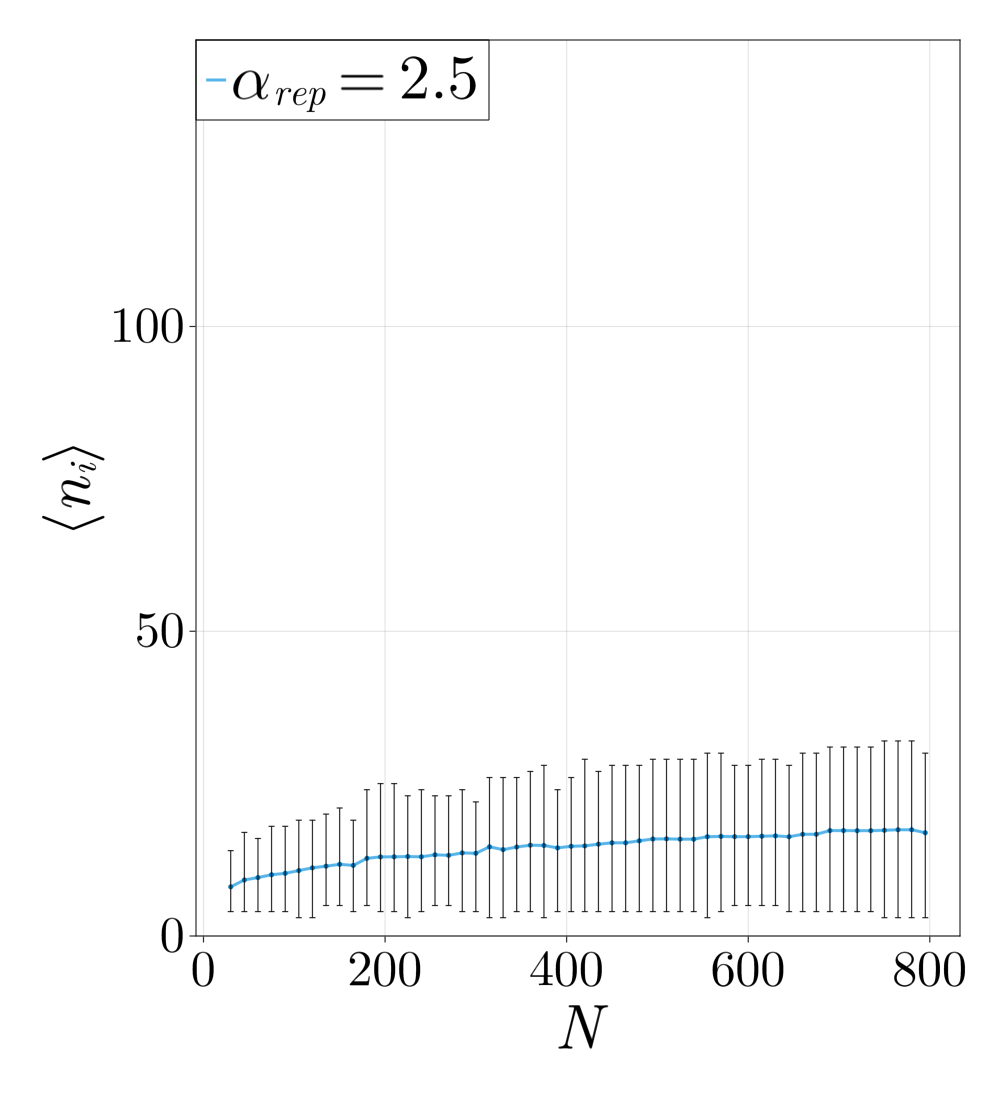
\includegraphics[width=\linewidth]{figures/303/303-reps-ni-2dot5.png} 
    \end{minipage}
    \begin{minipage}{0.49\textwidth}
        \centering
        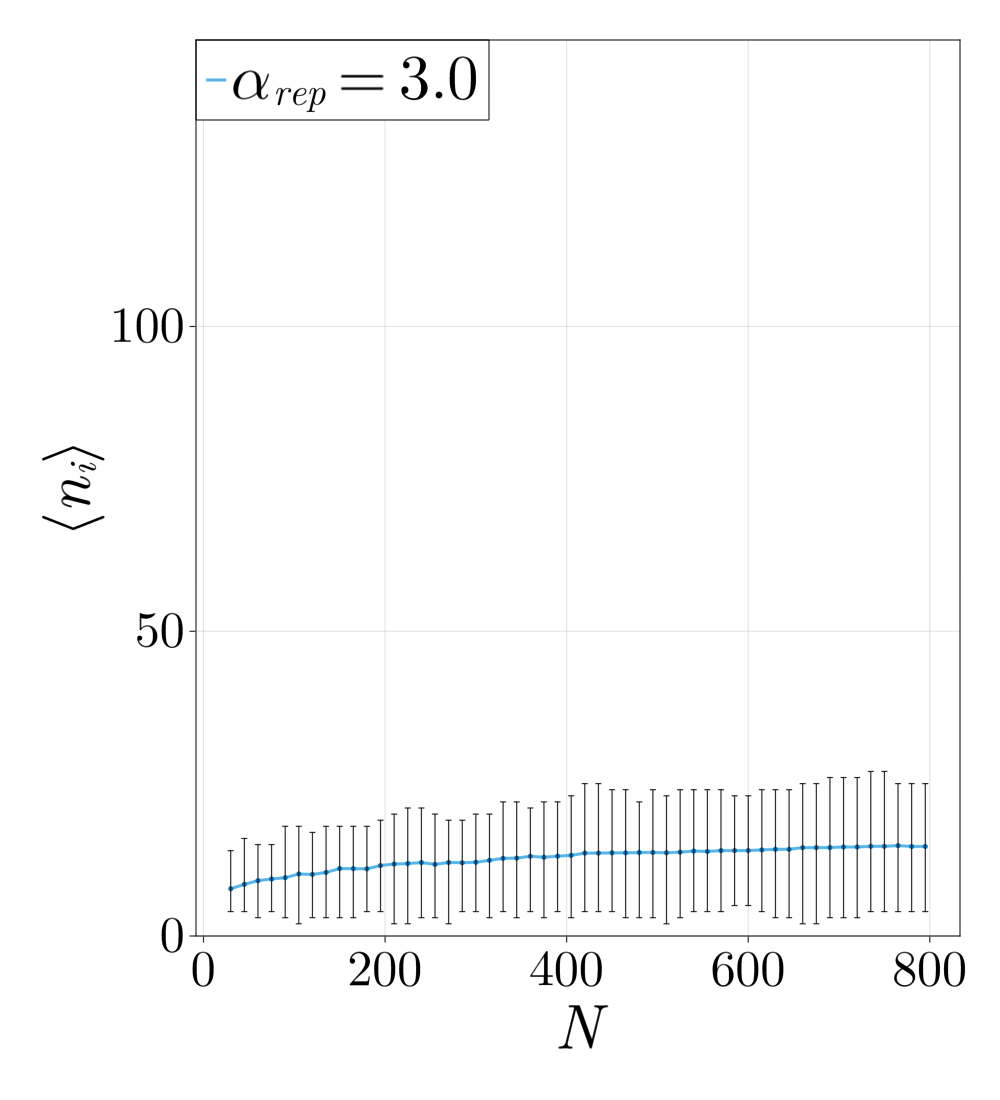
\includegraphics[width=\linewidth]{figures/303/303-reps-ni-3.png} 
    \end{minipage}

    \caption{Comparison of $\langle n_i \rangle$ for different values of $\alpha_\text{rep}$. Bars indicate the minimum and maximum number of neighbours for each $N$.}
    \label{fig:reps_ni_vs}
\end{figure}